\section{White Rabbit PTP}
\label{sec:wr}



\subsection{White Rabbit Synchronization}

White Rabbit is able to reach sub-nanoseconds accuracy and picoseconds
precision between two clocks:

\begin{itemize}
    \item Characterizing the asymmetry of the links 
    \item Measuring the phase shift of reference clock using clock loopback technique.
\end{itemize}

The \figurename~\ref{fig:wr_ptp} shows the WRPTP ~\cite{biblio:ispcs_m} flow and
its integration with the standard PTP . Bellow, a resume of the steps the WR synchronization 
process is outlined. A thoroughly description is presented in ~\cite{biblio:tomas} 
and ~\cite{biblio:wrptp}.

\subsubsection{Synthonization}

WRPTP initiates with a WR Announcement, in order to discover WR devices. 
If the other node is a WR device, the Lock procedure is triggered by the master.  
WRPTP uses SyncE to distribute a common frequency throughout. The slave will be 
frequency locked to the master. After what, both clocks will calibrate asymmetries 
present in the link. 

\subsubsection{Asymmetry Calibration}

WR calibrates the asymmetries in a optical link taking in consideration:

\begin{itemize}
    \item Fixed delays due to transmission circuitry
    \item Asymmetry of the optical transceivers and PHYs 
    \item Chromatic dispersion of the fiber optic    
\end{itemize}

\subsubsection{Coarse and Fine Delay Measurement}

After the calibration process, a first delay measurement, \textit{Coarse
Measurement} is issued using the Delay Request-Respond (DRR) mechanism. 
The next step towards the synchronization requires to figure out the phase shift
between the master and the looped-back clock from the sender, round trip 
phase shift, $phase_{mm}$. The ~\ref{fig:time_stamp} shows how between the 
master and the TC, the clock is looped back and the phase shift is measured 
using a phase detector, DDMTD ~\cite{biblio:ddmtd}. With the
$phase_{mm}$, the delay round trip, $delay_{mm}$ is calculated. The $phase_{s}$
is the phase shift of the clock adjustment derived form the $offset_ms$. Using the 
$phase_{mm}$ and $phase_{s}$ the timestamps on ingress ports can be enhanced, $t_{4p}$  $t_{2p}$,
using an algorithm described in ~\cite{biblio:tomas}.
Only timestamps on ingress ports need to bed enhanced, since they are generated 
asynchronously to the reference clock domain. The \textit{Fine Delay Measurement}, round trip,
is calculated as follows using now the enhanced timestamps :

\begin{equation}
  \label{eq:round_trip}
    delay_{mm} = (t_{4p} - t_1) - (t_3 - t_{2p})
\end{equation}

\subsubsection{Synchronization}

In order to finish the synchronization of the Slave clock to the Master Clock
the offset between both the clocks must be calculate, $offset_{MS}$. The round
trip can be expressed as function of the  delay master to slave, $\sigma _{ms}$ , slave to
master $sigma _{sm}$ and the sum of the fixed delays, $\delta$ , obtained during the calibration.

\begin{equation}
  \label{eq:round_trip_2}
    delay_{mm} = \Delta + \sigma _{ms} + \sigma _{sm}
\end{equation}

The ratio between single delays corresponds to the asymmetry of the propagation speed of
the different wavelength due to the chromatic dispersion, and is expressed:

\begin{equation}
    \label{eq:disp}
    (\alpha-1) = \frac{\sigma_{ms}}{\sigma_{sm}}
\end{equation}

From (\ref{eq:round_trip}), (\ref{eq:round_trip_2}) and  (\ref{eq:disp}) the delay
master to slave and $offset_{MS}$:

\begin{equation}
    \label{eq:delayms}
     delay_{ms} = \frac{1+ \alpha}{2+ \alpha}(delay_{mm} - \Delta)+ \Delta_{txm} + \Delta_{rxs} 
\end{equation}

\begin{equation}
    \label{eq:offsetms}
    offset_{ms} = t_{1} - t_{2p} - delay_{ms}
\end{equation}


After the initial WRPTP synchronization, a DDR or Peer Delay mechanism produces the 
timestamps, $t_{1}$, $t_{2p}$, $t_{3}$ and $t_{4p}$ (in case Peer Delay, also
$t_{5}$ and $t_{6p})$ and the DDMTD tracks changes in the $phase_{mm}$ over time. 

\begin{figure}[!t]
\centering
%\includegraphics[width=2.95in]{fig/wrCRS.eps}
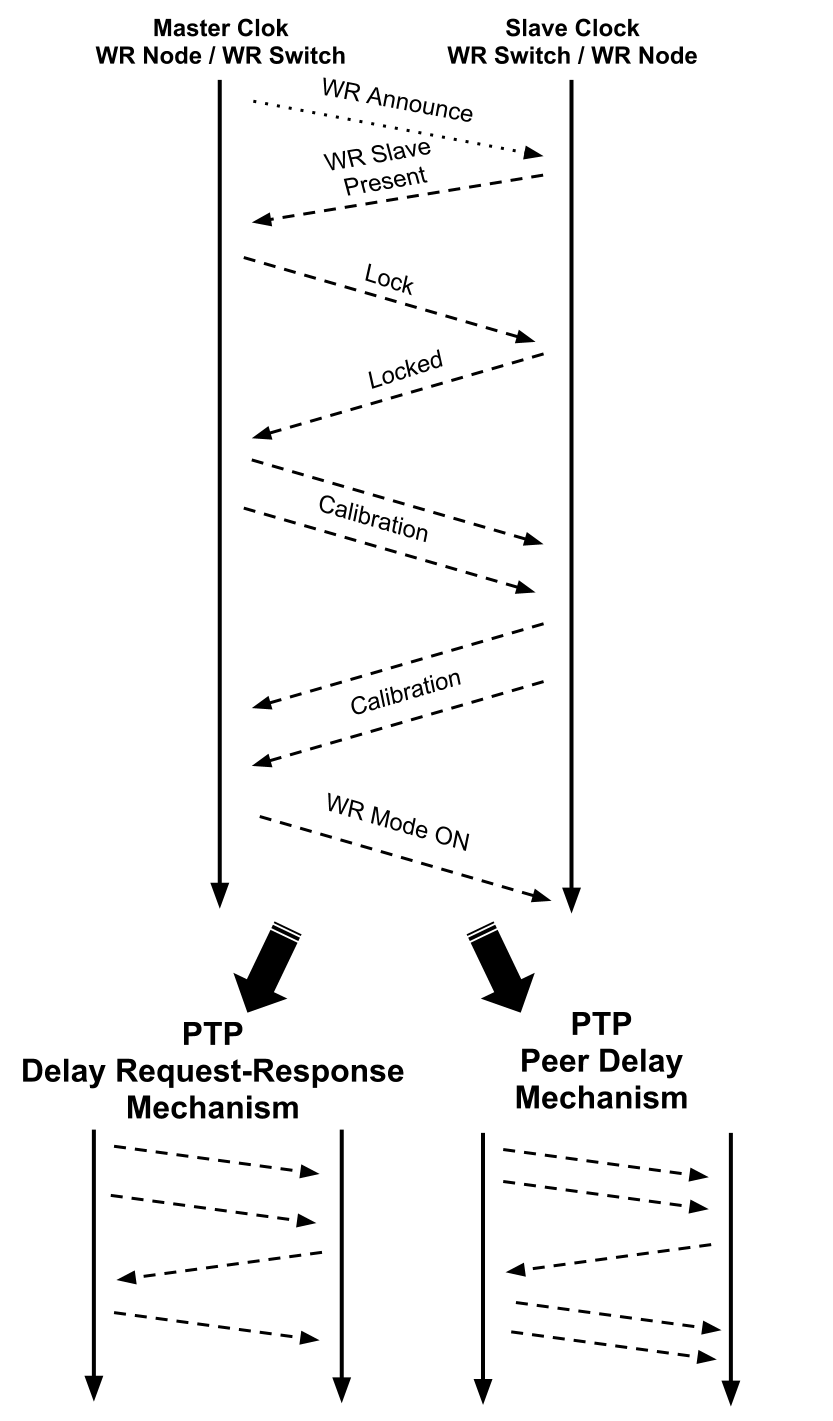
\includegraphics[scale=0.25]{fig/wr_ptp.png}
\caption{WR PTP Message Flow and PTP}
\label{fig:wr_ptp}
\end{figure}

%\FloatBarrier

